\section{Results and Discussions}
\label{sec:results}

We now present a thorough evaluation of \method~against both single-pass and multi-pass baseline methods, focusing on its ability to detect faithfulness and factuality hallucinations, as well as its computational efficiency. We further discuss notable trends and provide an assessment of areas where \method~is particularly effective, as well as scenarios where its advantages are less pronounced. The performance of \method~across four datasets and six models with $AUC_s$, $AUC_r$, $PCC_s$ and $PCC_r$ as evaluation metrics, compared against six baselines consisting of state-of-the-art single-pass and multi-pass detection techniques, are summarized in Table~\ref{tab:summary_results}, and the performance for individual datasets are further detailed in Table~\ref{tab:results_exp} of Appendix B. Further, the performances with AUC-ROC and PCC values calculated based on exact-match as the correctness measure are reported in Table~\ref{tab:exact_match} of Appendix C.

\begin{table*}[t!]
% \tiny
\centering
\adjustbox{width=\linewidth}{
\begin{tabular}{lcccc|cccc|cccc|cccc}
\toprule
Method 
& \multicolumn{4}{c}{RACE}
& \multicolumn{4}{c}{SQuAD}
& \multicolumn{4}{c}{NQ}
& \multicolumn{4}{c}{TriviaQA} \\
\cmidrule(lr){2-5} \cmidrule(lr){6-9} \cmidrule(lr){10-13} \cmidrule(lr){14-17}
& AUC$_s$ & AUC$_r$ & PCC$_s$ & PCC$_r$
& AUC$_s$ & AUC$_r$ & PCC$_s$ & PCC$_r$
& AUC$_s$ & AUC$_r$ & PCC$_s$ & PCC$_r$
& AUC$_s$ & AUC$_r$ & PCC$_s$ & PCC$_r$ \\
\hline

\multicolumn{17}{c}{\cellcolor[HTML]{C0C0C0}{Llama-3-8B}} \\ \hline
Probing 
& 67.25 & \textbf{67.54} & \textbf{26.54} & \textbf{34.60} & 68.79 & 69.83 & 37.06 & 37.68 & 75.27 & 76.07 & 41.86 & 32.14 & \textbf{85.18} & \textbf{87.68} & \textbf{77.42} & \textbf{70.81} \\
\textbf{\method} 
& \textbf{69.81} & 66.95 & 16.76 & 22.87 & \textbf{76.87} & \textbf{77.45} & \textbf{49.09} & \textbf{50.43} & \textbf{79.02} & \textbf{79.17} & \textbf{49.61} & \textbf{33.91} & 65.65 & 66.82 & 41.82 & 35.19 \\
\hline
\multicolumn{17}{c}{\cellcolor[HTML]{C0C0C0}{Llama-3-8B-Instruct}} \\ \hline
Probing 
& 70.83 & 68.16 & \textbf{33.15} & \textbf{37.61} & 62.88 & 62.52 & 27.15 & 26.34 & 76.70 & 77.35 & 47.20 & 35.74 & \textbf{84.88} & \textbf{86.95} & \textbf{75.67} & \textbf{66.77} \\
\textbf{\method} 
& \textbf{73.20} & \textbf{72.73} & 22.12 & 30.11 & \textbf{80.15} & \textbf{79.14} & \textbf{52.27} & \textbf{55.98} & \textbf{79.29} & \textbf{78.91} & \textbf{56.33} & \textbf{37.98} & 61.70 & 62.94 & 36.73 & 27.27 \\
\hline
\multicolumn{17}{c}{\cellcolor[HTML]{C0C0C0}{Gemma-2-9B}} \\ \hline
Probing 
& 57.92 & \textbf{58.25} & 15.71 & 13.47 & 69.25 & 70.36 & 36.51 & 38.15 & \textbf{85.97} & \textbf{84.32} & \textbf{24.44} & \textbf{16.55} & \textbf{86.70} & \textbf{87.28} & 47.67 & 40.62 \\
\textbf{\method} 
& \textbf{58.06} & 57.99 & \textbf{20.60} & \textbf{16.50} & \textbf{75.17} & \textbf{76.66} & \textbf{47.63} & \textbf{48.43} & 79.08 & 75.96 & 24.08 & 15.41 & 80.84 & 81.02 & \textbf{50.51} & \textbf{43.88} \\
\hline
\multicolumn{17}{c}{\cellcolor[HTML]{C0C0C0}{Gemma-2-9B-Instruct}} \\ \hline
Probing 
& \textbf{66.66} & \textbf{66.64} & \textbf{20.03} & \textbf{22.70} & 55.35 & 56.89 & 15.29 & 14.99 & 84.75 & 83.83 & 11.09 & 22.16 & \textbf{77.08} & \textbf{78.42} & -2.06 & 19.82 \\
\textbf{\method} 
& 64.18 & 64.03 & 11.92 & 16.26 & \textbf{72.69} & \textbf{73.32} & \textbf{39.73} & \textbf{39.70} & \textbf{85.19} & \textbf{85.89} & \textbf{51.20} & \textbf{41.99} & 70.90 & 70.72 & \textbf{52.64} & \textbf{45.90} \\

\bottomrule
\end{tabular}
}
\caption{
\changed{Comparison between supervised probing and \method~across four QA datasets.
Probing models are trained on TriviaQA and evaluated without retraining on other datasets.
Bold indicates the best-performing method per metric.
}}
\label{tab:probe_comparison}
\end{table*}



\changed{
\paragraph{Comparison with Supervised Probing Methods}
We additionally compare \method~against a supervised probing baseline following the state-of-the-art methodology of \citet{obeso2025realtimedetectionhallucinatedentities}. Specifically, we train a logistic regression classifier on token-level hidden states extracted from TriviaQA, using the same layer selection strategy as the original work, i.e., extracted from the middle layer. During inference, sequence-level hallucination scores are obtained by aggregating token-level predictions via maximum probability, ensuring sensitivity to localized hallucinated spans.
}
% \changed{
% While the trained probe achieves strong performance on its training domain, we observe that its performance degrades on unseen datasets. In contrast, \method~consistently outperforms the probe on RACE, SQuAD, and Natural Questions, highlighting the advantage of a training-free dependence-based criterion for cross-dataset generalization.
% }
\changed{
Table~\ref{tab:probe_comparison} compares \method~against a supervised probing baseline across four datasets and four large-scale LMs. As expected, probing performs strongly on its training distribution. For example, on TriviaQA, probing achieves AUC$_s$ scores of 85.18 and 84.88 on Llama-3-8B and Llama-3-8B-Instruct respectively, with correspondingly high PCC values, reflecting the benefit of supervised alignment.
}

\changed{
However, this advantage does not consistently transfer across datasets. On SQuAD, \method~outperforms probing across all four models, with gains exceeding 8 AUC points on Llama-3-8B (76.87 vs.\ 68.79) and nearly 18 points on Llama-3-8B-Instruct (80.15 vs.\ 62.88). Similar trends are observed on Natural Questions, where \method~achieves higher AUC$_s$ and PCC$_s$ across all models, including a +6 AUC gain on Gemma-2-9B and +25 PCC gain on Gemma-2-9B-Instruct.
}

\changed{
These results highlight a fundamental trade-off. While supervised probes excel when training and evaluation distributions align, their performance degrades under domain shift and requires labeled data and retraining to recover. In contrast, \method~operates entirely at inference time, requires no supervision, and demonstrates stronger cross-dataset generalization by directly measuring statistical dependence between input and output representations. This makes \method~particularly suitable for deployment scenarios where labeled hallucination data is unavailable or distribution shifts are expected.
}


\subsection{Faithfulness Hallucination Detection}
\label{sec:faithful_results}

Faithfulness hallucinations, characterized by outputs unsupported by the provided context, pose a critical challenge for reliable QA systems. Our results on SQuAD and RACE, as summarized in Tables~\ref{tab:results_exp} and~\ref{tab:exact_match}, demonstrate that \method~consistently outperforms single-pass baselines, such as Perplexity and Energy-score, in $10$ out of $12$ $(model, dataset)$ combinations. Across all models on SQuAD and RACE, \method~achieves respective average relative improvements of $47.4\%$ and $20.1\%$ in $AUC_s$ scores over the best-performing single-pass baseline.

\method's advantage persists when compared to the state-of-the-art multi-pass methods. On SQuAD, for example, \method~achieves an $AUC_s$ score of $80.15\%$ with Llama-3-8B-Instruct, which is an absolute improvement of $8$ percentage points over Eigenscore, the state-of-the-art multi-pass baseline. The improvements are also reflected in PCC values, with \method~outperforming single-pass baselines and matching the best multi-pass alternatives in most settings. This trend is also mirrored on the RACE dataset, where \method~provides consistently robust performance across both base and instruction-tuned variants of all models. Overall, for faithfulness hallucination detection, \method~achieves an average relative gain of $33.7\%$ and $6.5\%$ in $AUC_s$ over the  single-pass and multi-pass baselines, respectively. These results collectively underscore the effectiveness of measuring internal representational dependence as a robust strategy for detecting faithfulness hallucinations across diverse language model architectures and question-answering scenarios.

\begin{figure}[t!]
    \centering
    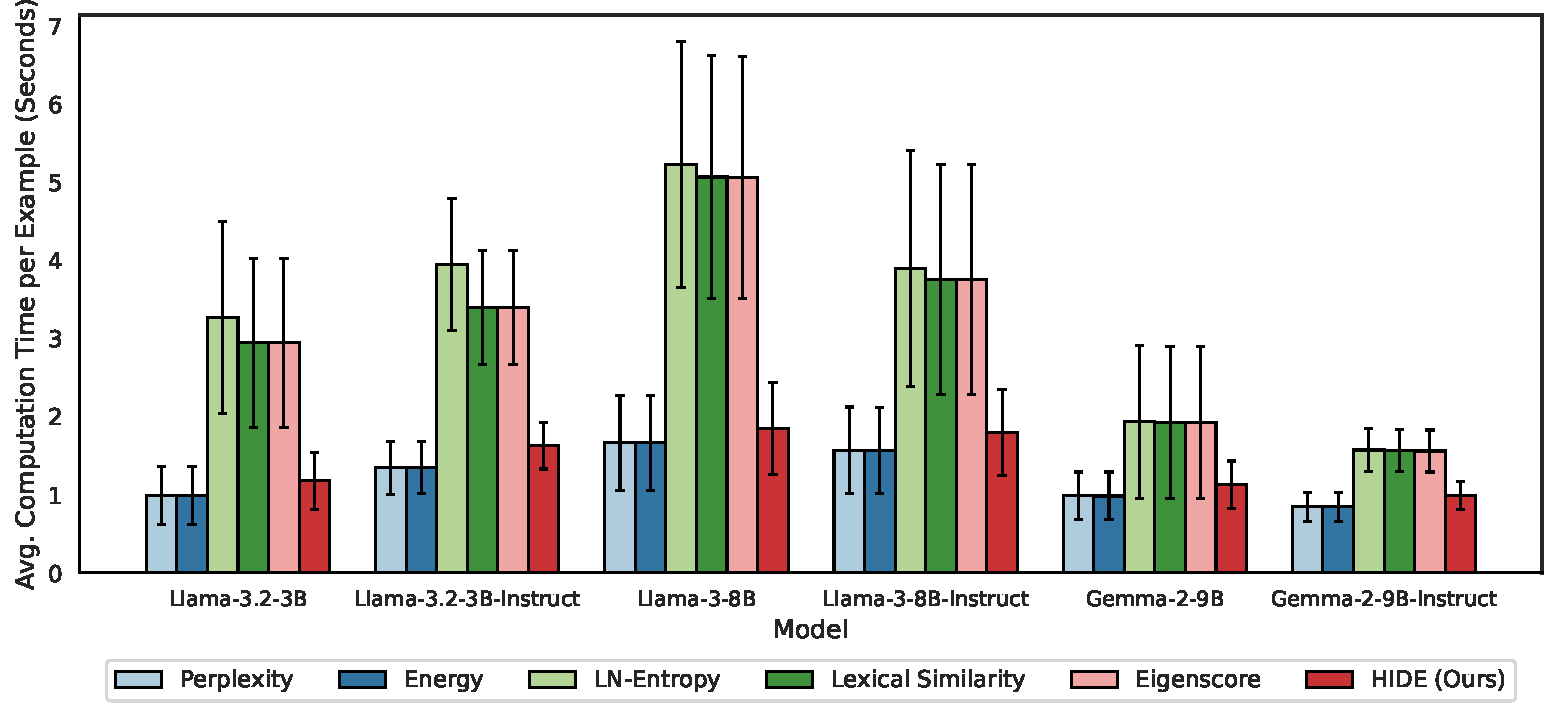
\includegraphics[width=\columnwidth]{files/figures/computation_time_plot.pdf}
    \caption{Comparison of the average computation time required by different hallucination detection methods to process each example, for six models. The averaging is done across all instances in the four datasets, i.e., RACE, SQuAD, NQ, and TriviaQA. \changedtwo{While consistency-based methods (Eigenscore, Lexical Similarity) incur a 2x--3x increase in latency due to repeated auto-regressive decoding, \method's single-pass design maintains a computational footprint comparable to standard uncertainty metrics in our benchmarking environment. These results represent a baseline architectural comparison; practical performance gains in production may be influenced by hardware-specific memory I/O constraints during the extraction of hidden states.}}
    \label{fig:time_analysis}
    \vspace{-5mm}
\end{figure}

\subsection{Factuality Hallucination Detection}
\label{sec:factual_results}

We further evaluate \method~on benchmarks designed to test factuality hallucinations, such as Natural Questions (NQ) and TriviaQA. Here, the outputs may be fluent yet factually unsupported. As shown in Tables~\ref{tab:results_exp} and~\ref{tab:exact_match}, even in the case of factuality hallucinations, \method~consistently provides improvements over single-pass baselines (in $10$ out of $12$ settings), with an average gain of $22.9\%$ in $AUC_s$ scores across models for NQ and TriviaQA. For instance, on NQ, \method~achieves $AUC_s$ score of $79.29\%$ with Llama-3-8B-Instruct, compared to $57.47\%$ for the best uncertainty-based single-pass competitor. The method also provides higher PCC values, indicating greater consistency with ground-truth correctness.

Compared to multi-pass methods, \method~is generally competitive and, in some settings, outperforms both Eigenscore and Lexical Similarity. For example, on the NQ dataset, \method~achieves higher AUC-ROC and PCC scores than all other methods for all six model variants. However, in certain configurations, such as TriviaQA with Llama-3-8B, the advantage of \method~is less pronounced, and Eigenscore achieves marginally higher AUC-ROC and PCC values. A closer examination of these cases suggests that datasets with extremely short or repetitive answers can reduce the discriminative power of representation-based dependence measures. We discuss such limitations in detail in \cref{sec:error_analysis}.


\begin{table*}[t!]
\tiny
\centering
% \adjustbox{width=0\linewidth}{
{
\begin{tabular}{lcc}
\toprule
\multirow{2}{*}{Method}
& \multicolumn{2}{c}{\textbf{HaluEval (Dialogue)}} \\
\cmidrule(lr){2-3}
& AUC$_s$ & AUC$_r$ \\
%%%%%%%%%%%%%%%%%%%%%%%%%%%%%%%%%%%%%%%%%%%%%%%%%%%%%%%%%%%%%%%%%%%%%%%%%%%%%%%%%%%%%%%%%%%%%%
\hline
\multicolumn{3}{c}{\cellcolor[HTML]{C0C0C0}Llama-3.2-3B} \\\hline
Perplexity & 68.00 & \underline{\textbf{72.00}} \\
Energy & 62.00 & 66.00 \\
\rowcolor{gray!20} LN-Entropy & 68.00 & 68.00 \\
\rowcolor{gray!20} Lexical Similarity & \textbf{75.00} & \textbf{72.00} \\
\rowcolor{gray!20} Eigenscore & 64.00 & 61.00 \\
\method & \underline{70.00} & 57.00 \\
%%%%%%%%%%%%%%%%%%%%%%%%%%%%%%%%%%%%%%%%%%%%%%%%%%%%%%%%%%%%%%%%%%%%%%%%%%%%%%%%%%%%%%%%%%%%%%
\hline
\multicolumn{3}{c}{\cellcolor[HTML]{C0C0C0}Llama-3.2-3B-Instruct} \\\hline
Perplexity & \underline{68.00} & \underline{\textbf{72.00}} \\
Energy & 58.00 & 57.00 \\
\rowcolor{gray!20} LN-Entropy & 67.00 & 69.00 \\
\rowcolor{gray!20} Lexical Similarity & \textbf{69.00} & \textbf{72.00} \\
\rowcolor{gray!20} Eigenscore & 65.00 & 64.00 \\
\method & 63.00 & 59.00 \\
%%%%%%%%%%%%%%%%%%%%%%%%%%%%%%%%%%%%%%%%%%%%%%%%%%%%%%%%%%%%%%%%%%%%%%%%%%%%%%%%%%%%%%%%%%%%%%
\hline
\multicolumn{3}{c}{\cellcolor[HTML]{C0C0C0}Llama-3-8B} \\\hline
Perplexity & 62.00 & \underline{\textbf{68.00}} \\
Energy & 57.00 & 63.00 \\
\rowcolor{gray!20} LN-Entropy & 61.00 & 62.00 \\
\rowcolor{gray!20} Lexical Similarity & \textbf{66.00} & \textbf{68.00} \\
\rowcolor{gray!20} Eigenscore & 61.00 & 58.00 \\
\method & \underline{\textbf{66.00}} & 55.00 \\
%%%%%%%%%%%%%%%%%%%%%%%%%%%%%%%%%%%%%%%%%%%%%%%%%%%%%%%%%%%%%%%%%%%%%%%%%%%%%%%%%%%%%%%%%%%%%%
\hline
\multicolumn{3}{c}{\cellcolor[HTML]{C0C0C0}Llama-3-8B-Instruct} \\\hline
Perplexity & \underline{64.00} & \underline{\textbf{70.00}} \\
Energy & 56.00 & 62.00 \\
\rowcolor{gray!20} LN-Entropy & 65.00 & 67.00 \\
\rowcolor{gray!20} Lexical Similarity & \textbf{66.00} & \textbf{70.00} \\
\rowcolor{gray!20} Eigenscore & 60.00 & 59.00 \\
\method & 61.00 & 55.00 \\
%%%%%%%%%%%%%%%%%%%%%%%%%%%%%%%%%%%%%%%%%%%%%%%%%%%%%%%%%%%%%%%%%%%%%%%%%%%%%%%%%%%%%%%%%%%%%%
\hline
\multicolumn{3}{c}{\cellcolor[HTML]{C0C0C0}Gemma-2-9B} \\\hline
Perplexity & \underline{73.00} & \underline{\textbf{73.00}} \\
Energy & 43.00 & 39.00 \\
\rowcolor{gray!20} LN-Entropy & 72.00 & 71.00 \\
\rowcolor{gray!20} Lexical Similarity & 75.00 & \textbf{73.00} \\
\rowcolor{gray!20} Eigenscore & \textbf{78.00} & 72.00 \\
\method & 64.00 & 53.00 \\
%%%%%%%%%%%%%%%%%%%%%%%%%%%%%%%%%%%%%%%%%%%%%%%%%%%%%%%%%%%%%%%%%%%%%%%%%%%%%%%%%%%%%%%%%%%%%%
\hline
\multicolumn{3}{c}{\cellcolor[HTML]{C0C0C0}Gemma-2-9B-Instruct} \\\hline
Perplexity & \underline{\textbf{71.00}} & \underline{\textbf{73.00}} \\
Energy & 42.00 & 43.00 \\
\rowcolor{gray!20} LN-Entropy & 68.00 & 71.00 \\
\rowcolor{gray!20} Lexical Similarity & 67.00 & 72.00 \\
\rowcolor{gray!20} Eigenscore & 69.00 & 71.00 \\
\method & 56.00 & 54.00 \\
%%%%%%%%%%%%%%%%%%%%%%%%%%%%%%%%%%%%%%%%%%%%%%%%%%%%%%%%%%%%%%%%%%%%%%%%%%%%%%%%%%%%%%%%%%%%%%
\bottomrule
\end{tabular}
}
\caption{\changed{Dialogue hallucination detection results on the HaluEval benchmark. We report AUC-ROC using sentence similarity (AUC$_s$) and ROUGE-L (AUC$_r$) as correctness measures. Rows corresponding to multi-pass methods are highlighted in grey. The best result for each metric is shown in \textbf{bold}, while the best single-pass result is \underline{underlined}.}}
\label{tab:dialogue_results}
\vspace{-5mm}
\end{table*}



\subsection{Generalization to Conversational Hallucinations}
\label{sec:dialogue_results}
\changed{
To evaluate whether the representational decoupling hypothesis underlying HIDE extends beyond question answering, we examine its performance on the dialogue split of the HaluEval benchmark. In this setting, hallucinations typically manifest as inconsistencies with prior conversational context or unsupported factual claims, rather than incorrect answers to well-defined questions. Dialogue therefore provides a challenging testbed for assessing whether input--output representational dependence remains informative in more open-ended generation scenarios.
}

\changed{
Table~\ref{tab:dialogue_results} reports dialogue hallucination detection performance across six language models, including both base and instruction-tuned variants of Llama and Gemma. Overall, HIDE demonstrates competitive and often strong performance across models, particularly on larger architectures. For instance, on Llama-3-8B HIDE achieves the best $AUC_s$ score, substantially outperforming the uncertainty-based single-pass baselines and matching or exceeding multi-pass methods.
}

\changed{
At the same time, performance varies across models and metrics. On some smaller or instruction-tuned models, simpler signals such as lexical similarity or energy-based scores perform competitively, and in a few cases outperform HIDE on individual metrics. This variability highlights the increased difficulty of dialogue hallucination detection, where surface-level similarity or confidence cues may occasionally align with correctness.
}

\changed{
Taken together, these results suggest that representational decoupling captures a meaningful signal for conversational hallucinations, though dialogue remains a more challenging setting than QA. Rather than claiming universal dominance, we view these findings as evidence that HIDE generalizes beyond QA without additional supervision or inference-time overhead, while leaving room for complementary signals in particularly ambiguous conversational cases.
}


\subsection{Computational Efficiency}
\label{sec:compute_time}
% An important goal of \method~is to balance detection accuracy with computational efficiency. As illustrated in Figure~\ref{fig:time_analysis}, the average time required for computation of the \method~score is similar to other single-pass methods. We observe that \method~reduces computational time by approximately $51\%$ on average compared to methods requiring multiple generations, i.e., LN-Entropy, Lexical Similarity, and Eigenscore (we generated $5$ outputs corresponding to each input prompt for every multi-pass method). Notably, while Eigenscore demonstrates superior detection performance in certain scenarios, its computational requirements are substantially higher than \method~across all tested models. For instance, on Llama-3.2-3B-Instruct, Eigenscore requires approximately $3.4$ seconds per input compared to \method's $1.6$ seconds -- a $112.5\%$ increase in computation time. This disparity becomes even more pronounced with larger models, like Llama-3-8B, where the gap widens to as much as $2\times$ or even more for some configurations.
% The lower latency of \method, combined with its robust performance, supports its practical deployment in scenarios where both speed and accuracy are critical.
% \changed{\paragraph{Latency Measurement Protocol}
% To enable a fair, transparent, and reproducible comparison of inference-time costs, we conduct all latency measurements using the standard HuggingFace \texttt{transformers} library with a PyTorch backend on a single NVIDIA A100 (80GB) GPU. We intentionally avoid specialized serving engines such as vLLM, as their kernel-level optimizations vary substantially across model architectures (e.g., Llama versus Gemma) and could obscure method-level comparisons. Our objective is to isolate the intrinsic computational cost of hallucination detection strategies rather than report system-dependent optimizations.
% }
% \changed{\paragraph{Latency Accounting}
% For each method, we measure the end-to-end wall-clock time required to process a single input query, averaged over the full evaluation set. For \method, this latency includes standard auto-regressive generation, keyword extraction via KeyBERT, and HSIC computation. All measurements are performed under identical hardware and software conditions, ensuring that observed differences reflect algorithmic design choices rather than implementation artifacts.
% }
% \changed{\paragraph{Overhead Analysis}
% Auto-regressive generation constitutes the dominant inference bottleneck due to its strictly sequential nature. In contrast, the auxiliary components of \method -- namely keyword extraction and HSIC computation, are post-hoc operations that do not invoke additional decoding passes and therefore incur minimal overhead relative to generation. This distinction is confirmed quantitatively in our measurements. For example, on Llama-3-8B, generating a single output requires approximately 1.62 seconds on average, while the complete \method pipeline takes 1.71 seconds, corresponding to an overhead of only 0.09 seconds (approximately 5\%). In contrast, multi-pass methods that generate five outputs per input require approximately 5.50 seconds on average, making them roughly 3.4$\times$ slower under identical conditions.
% }
% \changed{\paragraph{Effect of Optimized Serving}
% While optimized inference engines such as vLLM can reduce wall-clock latency for generating multiple sequences through parallel sampling, they do not eliminate the fundamental increase in computational cost associated with decoding $k$ times more tokens. As a result, multi-pass methods necessarily incur higher FLOPs and memory bandwidth usage than single-generation approaches. Consequently, even under optimized serving stacks, methods requiring multiple generations remain asymptotically more expensive than \method, which performs hallucination detection using a single generation pass.
% }

% \changedtwo{\paragraph{Scalability and Overhead Analysis} 
% Auto-regressive generation constitutes the dominant inference bottleneck due to its strictly sequential nature. In contrast, the auxiliary components of \method~--namely keyword extraction and HSIC computation -- are post-hoc operations that do not invoke additional decoding passes and therefore incur minimal overhead relative to generation. For example, on Llama-3-8B, generating a single output requires approximately 1.62 seconds on average, while the complete \method~pipeline takes 1.71 seconds, corresponding to an absolute overhead of only 0.09 seconds (approximately 5\%). In contrast, multi-pass methods generating five outputs per input require approximately 5.50 seconds, making them roughly 3.4$\times$ slower under identical conditions.
% }

% \changedtwo{
% A critical design feature of \method~is that it computes statistical dependence on a fixed subset of representative tokens ($n_{eff}$) rather than the entire generated sequence. As a result, its computational complexity is decoupled from the total sequence length. Figure \ref{fig:scaling_latency} illustrates that the absolute latency of the \method~pipeline remains essentially flat at approximately $0.2$ seconds across varying effective token budgets. As the underlying generation takes longer for extended sequences, the relative overhead of \method~decays asymptotically toward zero. Furthermore, \method~scales efficiently with model size; the semantic extraction is model-agnostic, and the HSIC RBF kernel computation scales strictly linearly ($\mathcal{O}(d)$) with the hidden dimension $d$. As illustrated in Figure~\ref{fig:time_analysis}, transitioning from Llama-3.2-3B ($d=3072$) to Llama-3-8B ($d=4096$) yields an identical absolute pipeline overhead of approximately $0.23$ seconds, demonstrating a constant marginal cost scalable to larger architectures.
% }

% \changedtwo{\paragraph{Scalability and Overhead Analysis.} 
% Auto-regressive generation constitutes the dominant inference bottleneck due to its strictly sequential nature. In contrast, the auxiliary components of \method~-- namely keyword extraction and HSIC computation -- are post-hoc operations that do not invoke additional decoding passes and therefore incur minimal overhead relative to generation. For example, on Llama-3-8B, generating a single output requires approximately 1.62 seconds on average, while the complete \method~pipeline takes 1.71 seconds, corresponding to an absolute overhead of only 0.09 seconds (approximately 5\%). In contrast, multi-pass methods generating five outputs per input require approximately 5.50 seconds, making them roughly 3.4$\times$ slower under identical conditions.}

% \changedtwo{
% A critical design feature of \method~is that it computes statistical dependence on a fixed subset of representative tokens ($n_{eff}$) rather than the entire generated sequence. As a result, its computational complexity is decoupled from the total sequence length. Figure \ref{fig:scaling_latency}(a) illustrates that the absolute latency of the \method~pipeline remains essentially flat at approximately 0.2 seconds, demonstrating that the computation time is largely invariant to the chosen token budget ($n_{eff}$). As the underlying generation takes longer for extended sequences, the relative overhead of \method~ decays asymptotically toward zero, as shown in Figure \ref{fig:scaling_latency}(b). Furthermore, \method~ scales efficiently with model size; the semantic extraction is model-agnostic, and the HSIC RBF kernel computation scales strictly linearly ($\mathcal{O}(d)$) with the hidden dimension $d$. Transitioning from Llama-3.2-3B ($d=3072$) to Llama-3-8B ($d=4096$) yields an identical absolute pipeline overhead of approximately 0.23 seconds, demonstrating a constant marginal cost scalable to larger architectures.
% }

% \changedtwo{\paragraph{Inference Optimizations and System-Level Bottlenecks} 
% While optimized inference engines such as vLLM can reduce wall-clock latency for multiple sequences through parallel sampling, they do not eliminate the fundamental increase in computational cost associated with decoding $k$ times more tokens. Multi-pass methods necessarily incur higher FLOPs and memory bandwidth usage than single-generation approaches. Beyond these FLOP counts, modern serving engines present a structural barrier for multi-pass representation-based detection.}

% \changedtwo{
% Highly optimized engines achieve throughput by fusing kernels (e.g., PagedAttention) to keep computations within the GPU's SRAM, intentionally avoiding the materialization of intermediate hidden states to High Bandwidth Memory (HBM). To deploy any white-box detection method, the system must be modified to dump these hidden states to HBM for every generated token. Because LLM inference is primarily memory-bound, extracting states for $N$ independent responses creates a compounding I/O bottleneck that drastically inflates serving latency. Since \method~requires state extraction for only a single generation pass, it structurally avoids this compounding memory delay, offering a fundamental architectural advantage in production environments.} 

\changedtwo{\paragraph{Latency Measurement Protocol}
To characterize the baseline computational profile of different detection strategies, we conduct all latency measurements using the standard HuggingFace \texttt{transformers} library with a PyTorch backend on a single NVIDIA A100 (80GB) GPU. We utilize this standard environment to isolate the intrinsic algorithmic overhead of each method from system-level optimizations. While specialized serving engines offer significant throughput gains for standard generation, they often present structural barriers for representation-based detection. Highly optimized engines typically fuse kernels to keep computations within the GPU's SRAM; consequently, extracting hidden states for white-box methods would necessitate materializing these states to High Bandwidth Memory (HBM), potentially incurring a system-dependent I/O penalty.
}

\changedtwo{\paragraph{Latency Accounting}
For each method, we measure the end-to-end wall-clock time required to process a single input query, averaged over the full evaluation set. For \method, this latency encompasses the standard auto-regressive generation, keyword extraction via KeyBERT, and the modified HSIC computation. To ensure a fair baseline comparison, our measurements for multi-pass methods utilize optimized batched generation (via the \texttt{num\_return\_sequences} parameter) to compute multiple responses in parallel; thus, the multi-pass baselines are not artificially penalized by sequential decoding loops.
}

\changedtwo{\paragraph{Scalability and Overhead Analysis} 
Auto-regressive generation remains the primary inference bottleneck due to its sequential nature. In our standard benchmarking environment, the auxiliary components of \method~incur marginal overhead relative to generation. For Llama-3-8B, the base generation requires approximately $1.62$ seconds on average, while the complete \method~pipeline takes $1.71$ seconds, representing a marginal absolute overhead of $0.09$ seconds ($\approx 5\%$).}

\changedtwo{
A critical design feature of \method~ is that it computes statistical dependence on a fixed subset of representative tokens ($n_{eff}$) rather than the entire sequence. As a result, its computational complexity is largely decoupled from total sequence length. Figure \ref{fig:scaling_latency}(a) illustrates that the absolute latency of the \method~pipeline remains essentially flat at approximately $0.2$ seconds, demonstrating that computation time is invariant to the chosen token budget ($n_{eff}$). As the underlying generation takes longer for extended sequences, the relative overhead of \method~becomes negligible, as shown in Figure \ref{fig:scaling_latency}(b). Furthermore, \method~scales linearly with model size; semantic extraction is model-agnostic, and the HSIC computation scales linearly ($\mathcal{O}(d)$) with the hidden dimension $d$. Transitioning from Llama-3.2-3B ($d=3072$) to Llama-3-8B ($d=4096$) yields an identical absolute pipeline overhead of approximately $0.23$ seconds.
}

\changedtwo{\paragraph{Inference Optimizations and System-Level Bottlenecks} 
While optimized inference engines can reduce wall-clock latency through parallel sampling, they do not eliminate the structural increase in computational cost associated with decoding $k$ times more tokens. Multi-pass methods necessarily incur higher FLOPs and memory bandwidth usage than single-generation approaches. As noted previously, highly optimized engines achieve throughput by avoiding the materialization of intermediate hidden states to HBM. Because LLM inference is primarily memory-bound, extracting states for $N$ independent responses creates a compounding I/O bottleneck that inflates serving latency. Since \method~requires state extraction for only a single generation pass, it avoids this compounding delay, offering a structural architectural advantage in production environments.
}

\begin{figure}[t]
    \centering
    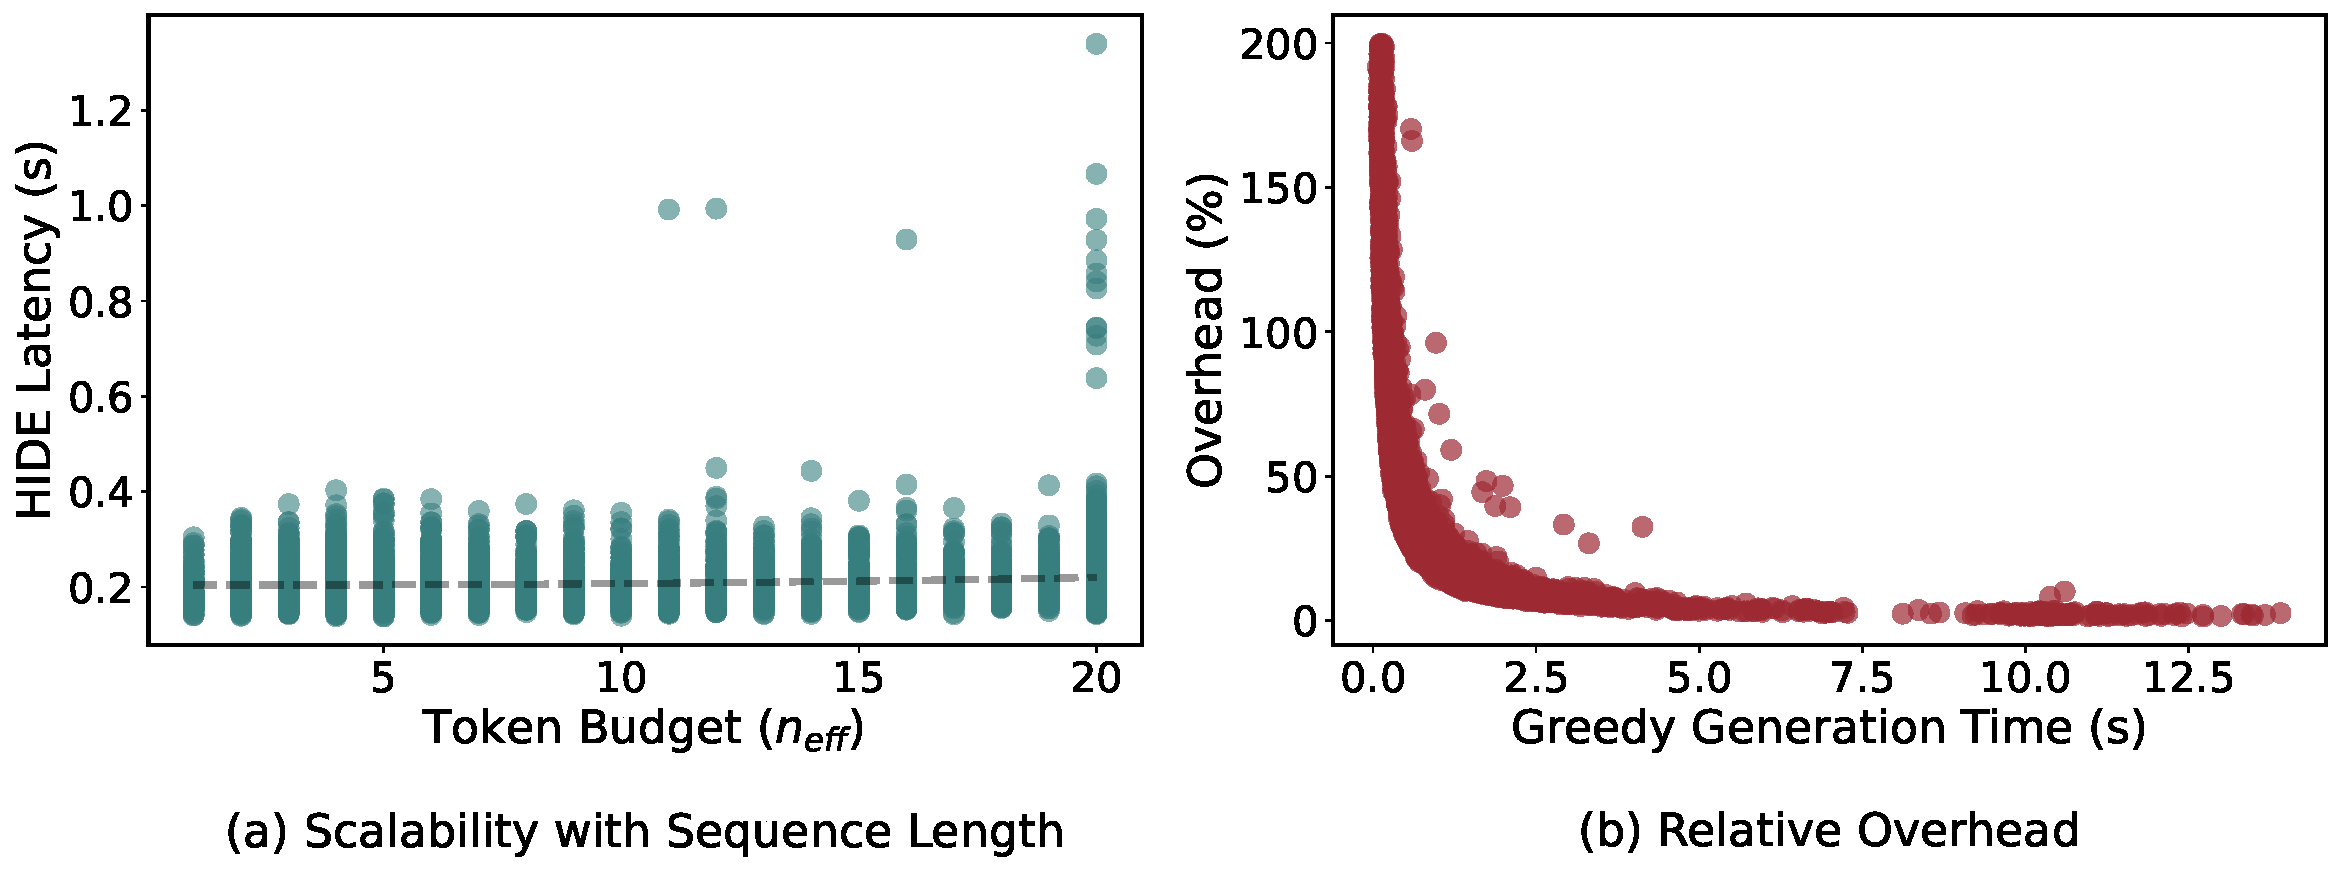
\includegraphics[width=\columnwidth]{files/figures/Scalability_Analysis.pdf} 
    \caption{\changedtwo{Scalability analysis of the \method~ framework. (a) Absolute latency of \method~ remains essentially constant regardless of the token budget ($n_{eff}$), ensuring efficiency even as the budget increases. (b) The relative overhead of \method~ drops asymptotically as the base generation time increases, rendering the computational cost negligible for standard outputs.}}
    \label{fig:scaling_latency}
\end{figure}

\changedtwo{\paragraph{Empirical Comparison Across Methods}
Figure~\ref{fig:time_analysis} summarizes these trends across the evaluated models and datasets. In our standard benchmarking environment, \method~provides a baseline reduction in computation time of approximately $51$\% compared to multi-pass approaches (where five outputs are generated per input). While remaining comparable in latency to other single-pass baselines, \method~exhibits significantly lower computational requirements than multi-pass state-of-the-art methods. For instance, on Llama-3.2-3B-Instruct, Eigenscore requires approximately $3.4$ seconds per input compared to $1.6$ seconds for \method, representing a measurable increase in latency. This gap remains consistent or increases for larger models such as Llama-3-8B, where the latency difference approaches or exceeds $2\times$ in several configurations.
}

\changedtwo{Taken together, these results indicate that \method~achieves a favorable balance between detection accuracy and computational overhead in standard inference settings. Its auxiliary computations introduce marginal overhead relative to the generation process, and its single-pass design yields measurable latency reductions over consistency-based multi-pass alternatives. While these baseline gains are promising, we emphasize that practical efficiency in production environments is subject to hardware-level memory I/O constraints, particularly during the extraction of hidden states from highly optimized inference kernels. Nonetheless, the architectural design of \method~provides a structural advantage for hallucination detection where both speed and reliability are critical.}

% \changed{\paragraph{Empirical Comparison Across Methods}
% Figure~\ref{fig:time_analysis} summarizes these trends across models and datasets. On average, \method~reduces computation time by approximately 51\% compared to multi-pass approaches such as LN-Entropy, Lexical Similarity, and Eigenscore (for which five outputs are generated per input), while remaining comparable in latency to other single-pass baselines. Although Eigenscore achieves strong detection performance in certain scenarios, its computational requirements are consistently higher than \method~across all tested models. For instance, on Llama-3.2-3B-Instruct, Eigenscore requires approximately 3.4 seconds per input compared to \method’s 1.6 seconds, representing a 112.5\% increase in computation time. This gap becomes even more pronounced for larger models such as Llama-3-8B, where the slowdown approaches or exceeds $2\times$ in some configurations.
% }

% \changed{Taken together, these results demonstrate that \method~achieves a favorable balance between detection accuracy and computational efficiency. Its auxiliary computations introduce negligible overhead relative to generation, and its single-pass design yields substantial latency reductions over consistency-based multi-pass alternatives, supporting its practical deployment in settings where both speed and reliability are critical.
% }


\subsection{Interpreting the \method~Score for Hallucination Detection}
\label{sec:interpreting-hide}

\begin{table*}[t!]
\centering
\adjustbox{width=0.6\linewidth}{
\begin{tabular}{lcccc|c}
\toprule
\multirow{2}{*}{\textbf{Model}} & \multicolumn{2}{c}{\textbf{Faithfulness}} 
& \multicolumn{2}{c}{\textbf{Factuality}} \\
\cmidrule(lr){2-3} \cmidrule(lr){4-5}
& RACE & SQuAD & NQ & TriviaQA & {\textbf{Average}}\\
%\cmidrule(lr){2-3} \cmidrule(lr){4-5} \cmidrule(lr){6-7} \cmidrule(lr){8-9} \cmidrule(lr){10-11}
% & $\text{AUC}$ & $\text{PCC}$ & $\text{AUC}$ & $\text{PCC}$& $\text{AUC}$ & $\text{PCC}$& $\text{AUC}$ & $\text{PCC}$ & $\text{AUC}$ & $\text{PCC}$\\
%%%%%%%%%%%%%%%%%%%%%%%%%%%%%%%%%%%%%%%%%%%%%%%%%%%%%%%%%%%%%%%%%%%%%%%%%%%%%%%%%%%%%%%%%%%%%%
\hline
% \multicolumn{4}{c}{\cellcolor[HTML]{C0C0C0}Llama-3.2-3B} \\\hline
Llama-3.2-3B& 0.10 & 0.12 & 0.14 & 0.19 & \changed{0.14} \\
%%%%%%%%%%%%%%%%%%%%%%%%%%%%%%%%%%%%%%%%%%%%%%%%%%%%%%%%%%%%%%%%%%%%%%%%%%%%%%%%%%%%%%%%%%%%%%
% \hline
% \multicolumn{4}{c}{\cellcolor[HTML]{C0C0C0}Llama-3.2-3B-Instruct} \\\hline
Llama-3.2-3B-Instruct&0.09 & 0.14 & 0.12 & 0.16 & \changed{0.13} \\
%%%%%%%%%%%%%%%%%%%%%%%%%%%%%%%%%%%%%%%%%%%%%%%%%%%%%%%%%%%%%%%%%%%%%%%%%%%%%%%%%%%%%%%%%%%%%%
% \hline
% \multicolumn{4}{c}{\cellcolor[HTML]{C0C0C0}Llama-3-8B} \\\hline
Llama-3-8B&0.09 & 0.12 & 0.14 & 0.16 & \changed{0.13} \\
%%%%%%%%%%%%%%%%%%%%%%%%%%%%%%%%%%%%%%%%%%%%%%%%%%%%%%%%%%%%%%%%%%%%%%%%%%%%%%%%%%%%%%%%%%%%%%
% \hline
% \multicolumn{4}{c}{\cellcolor[HTML]{C0C0C0}Llama-3-8B-Instruct} \\\hline
Llama-3-8B-Instruct& 0.09 & 0.12 & 0.16 & 0.16 & \changed{0.13}\\ %%%%%%%%%%%%%%%%%%%%%%%%%%%%%%%%%%%%%%%%%%%%%%%%%%%%%%%%%%%%%%%%%%%%%%%%%%%%%%%%%%%%%%%%%%%%%%
% \hline
% \multicolumn{4}{c}{\cellcolor[HTML]{C0C0C0}Gemma-2-9B} \\\hline
Gemma-2-9B & 0.11 & 0.10 & 0.12 & 0.12 & \changed{0.11}\\
%%%%%%%%%%%%%%%%%%%%%%%%%%%%%%%%%%%%%%%%%%%%%%%%%%%%%%%%%%%%%%%%%%%%%%%%%%%%%%%%%%%%%%%%%%%%%
% \hline
% \multicolumn{4}{c}{\cellcolor[HTML]{C0C0C0}Gemma-2-9B-Instruct} \\\hline
Gemma-2-9B-Instruct & 0.08	&0.10	&0.09	&0.10 & \changed{0.09}\\
\hline
\textbf{Average} & 0.09 & 0.11 & 0.13 & 0.15 & \changed{0.12}\\
\midrule
\end{tabular}
}
\caption{Threshold values for various settings using exact match as the correctness measure.}
\label{tab:threshold_values}
\end{table*}

% The output of the \method~framework is the \method~score, which quantifies the degree of statistical dependence between the internal representations of the input prompt and the output sequence generated by an LM. Interpreting this score effectively is essential for deploying \method~as a reliable tool for hallucination detection in practice.

% In order to enable a binary decision of whether a given model generation is hallucinated or not, we need to convert the continuous \method~score into a decision by applying a threshold. Intuitively, a lower \method~score signals a decoupling between the representations of input and output, suggesting a higher likelihood that the output is a hallucination. Conversely, a higher \method~score reflects a strong coupling, consistent with outputs that are faithful to the input or grounded in factual knowledge.

% \changed{
% \paragraph{Threshold Selection via Balanced Operating Point.}
% To convert the continuous \method~score into a binary hallucination decision, we require a threshold $\tau$ that separates hallucinated from faithful generations. Rather than optimizing for accuracy—which can be misleading under class imbalance—we treat threshold calibration as a trade-off between sensitivity (detecting hallucinations) and specificity (avoiding false alarms on correct outputs).
% }
% \changed{
% Concretely, we select $\tau$ by maximizing the Geometric Mean (G-Mean) of the True Positive Rate (TPR) and True Negative Rate (TNR):
% \[
% \text{G-Mean} = \sqrt{\text{TPR} \times \text{TNR}} = \sqrt{\text{TPR} \times (1 - \text{FPR})}.
% \]
% We sweep $\tau$ over the range of observed \method~scores on a validation set and select the value that maximizes G-Mean. This criterion penalizes extreme failure in either direction and yields a balanced operating point even when hallucinations are rare.
% }

% \paragraph{\textbf{Empirical Threshold Determination}}
% We analyze the average value of threshold, $\tau_{\mathrm{avg}}$, from our diverse evaluation setup spanning four benchmark datasets and six models. When utilizing the \method~framework, the condition, $\widehat{\operatorname{HSIC}}_{\method} < \tau_{\mathrm{avg}}$, would thus potentially indicate a hallucinated generation.


% For each $(dataset, model)$ pair, we identify the threshold that most effectively separates the hallucinated outputs from non-hallucinated ones, by maximizing $\text{G-Mean}=
% \sqrt{\mathrm{TPR}\times(1-\mathrm{FPR})}$, using the exact match labels after comparison with ground-truth, indicating whether the generation is hallucinated or not. Here, $\mathrm{TPR}$ and  $\mathrm{FPR}$ denote  true-positive and false-positive rates, respectively.  G-Mean  thus combines sensitivity and specificity into one value penalizing classifiers that perform well on one class but poorly on another, making it suitable for imbalanced datasets where accuracy alone can be misleading.

% Across all four evaluated datasets, i.e., SQuAD, RACE, Natural Questions, and TriviaQA, and the six LMs considered in our experiments, we find that the optimal thresholds are mostly consistent, as shown in Table~\ref{tab:threshold_values}, yielding an average threshold value $\tau_{\mathrm{avg}} = 0.12$. Our observation suggests that the \method~score has a stable behaviour across diverse tasks and models. We provide examples of a few input prompts from various datasets and the corresponding generations from Llama-3-8B along with the respective \method~scores in Appendix C, to illustrate how hallucinated generations are detected by \method.

% \subsection{Interpreting the \method~Score for Hallucination Detection}
% \label{sec:threshold}

\changed{
\method~produces a continuous-valued score that reflects the degree of statistical dependence between input and output representations. Lower scores indicate stronger representational decoupling and thus a higher likelihood of hallucination. To operationalize this signal for hallucination detection, the score must be converted into a binary decision using a threshold $\tau$. In this section, we describe how $\tau$ is selected, analyze its stability across models, and discuss its interpretation in deployment settings.
}

\changed{
\paragraph{Threshold Selection via Balanced Operating Point}
Selecting an appropriate threshold $\tau$ involves balancing two competing objectives: sensitivity (detecting hallucinated generations) and specificity (avoiding false alarms on faithful outputs). Optimizing for accuracy alone can be misleading, particularly under class imbalance, as it may bias the threshold toward the majority class. To avoid this, we select $\tau$ by maximizing the Geometric Mean (G-Mean) of the True Positive Rate (TPR) and the True Negative Rate (TNR):
\[
\text{G-Mean} = \sqrt{\text{TPR} \times \text{TNR}} = \sqrt{\text{TPR} \times (1 - \text{FPR})}.
\]
We sweep $\tau$ over the range of observed \method~scores on a validation set and select the value that maximizes G-Mean. This criterion penalizes extreme failure in either direction and yields a balanced operating point, even when hallucinations constitute a minority of the data.
}

% \changed{
% \paragraph{Threshold Stability Across Model Variants and Datasets}
% Table~\ref{tab:threshold_values} reports the optimal thresholds obtained via G-Mean optimization across datasets and model variants. We observe that $\tau$ remains stable across base and instruction-tuned versions of the same architecture. For example, the optimal threshold for Llama-3-8B is 0.13 for both base and instruct variants, while Llama-3.2-3B exhibits thresholds of 0.14 (base) and 0.13 (instruct). Similarly, Gemma-2-9B yields closely aligned thresholds of 0.11 (base) and 0.09 (instruct). We also observe that across all four evaluated datasets, i.e., SQuAD, RACE, Natural Questions, and TriviaQA, the optimal thresholds are mostly consistent, as shown in Table~\ref{tab:threshold_values}, yielding an average threshold value $\tau_{\mathrm{avg}} = 0.12$. This consistency suggests that the representational decoupling captured by \method~reflects a structural property of the model that is largely preserved during instruction tuning, rather than a dataset- or training-specific artefact.}We provide examples of a few input prompts from various datasets and the corresponding generations from Llama-3-8B along with the respective \method~scores in Appendix C, to illustrate how hallucinated generations are detected by \method.

\changed{
\paragraph{Variance of the Optimal Threshold}
Beyond the consistency of the average optimal threshold ($\tau_{\text{avg}} \approx 0.12$), we further analyze the variance of $\tau$ across datasets and model variants to assess deployment stability. Overall, we observe that the optimal threshold remains largely consistent between base and instruction-tuned models. For example, Llama-3-8B exhibits an average optimal threshold of $\tau = 0.13$ for both its Base and Instruct variants, while Llama-3.2-3B shows similarly close values ($\tau = 0.14$ for Base and $\tau = 0.13$ for Instruct). Gemma-2-9B follows the same pattern, with $\tau = 0.11$ for the Base model and $\tau = 0.09$ for the Instruct variant. We also observe that across all four evaluated datasets, i.e., SQuAD, RACE, Natural Questions, and TriviaQA, the optimal thresholds are mostly consistent, as shown in Table~\ref{tab:threshold_values}, yielding an average threshold value $\tau_{\mathrm{avg}} = 0.12$. This suggests that the representational decoupling signal captured by \method~is structural and largely preserved under instruction tuning.
}We provide examples of a few input prompts from various datasets and the corresponding generations from Llama-3-8B along with the respective \method~scores in Appendix D, to illustrate how hallucinated generations are detected by \method.

\changed{
Analyzing variance across datasets reveals a more nuanced picture. Instruction-tuned models often exhibit lower threshold variance than their base counterparts -- e.g., Llama-3.2-3B-Instruct shows a variance of $0.00087$ compared to $0.00141$ for its Base version, and Gemma-2-9B-Instruct shows a variance of $0.00005$ versus $0.00012$ for Gemma-2-9B Base. However, this trend is not universal: Llama-3-8B-Instruct exhibits slightly higher variance ($0.00114$) than its Base version ($0.00087$). These results indicate that while instruction tuning often stabilizes the optimal threshold, the effect is model-family dependent.
}


\changed{
Taken together, these findings suggest that HIDE admits a largely stable operating threshold across both model variants and datasets, supporting practical deployment with minimal per-model calibration. At the same time, the observed variance patterns motivate lightweight validation-based calibration when deploying across substantially different model families.
}

\changed{
\paragraph{Interpreting $\tau$ in Deployment}
The threshold $\tau$ selected during validation defines a default operating point for inference: generations with \method~scores below $\tau$ are flagged as hallucinated. In practice, however, $\tau$ can be adjusted to reflect application-specific risk preferences. In safety-critical domains, such as medical or legal assistance, practitioners may lower $\tau$ to prioritize recall, accepting a higher false positive rate in order to minimize undetected hallucinations. Conversely, in user-experience-sensitive applications, such as creative writing or casual dialogue, a higher $\tau$ may be preferred to reduce unnecessary flags on correct outputs. Accordingly, while the G-Mean–optimized threshold provides a principled and balanced baseline, $\tau$ should be viewed as a tunable operating parameter rather than a fixed constant.
}


